
\section{Durchführung}
\label{sec:Durchführung}
\subsection{Aufbau}
\label{sec:Aufbau}

\begin{figure}[H]
  \centering
  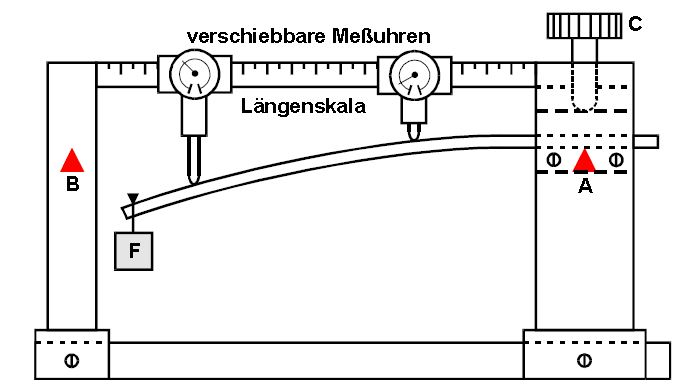
\includegraphics[width=\linewidth-30pt,height=\textheight-30pt,keepaspectratio]{Text/Bilder/Aufbau.png}
  \caption{Schematische Darstellung der kompletten Messapparatur \cite[13]{sample}.}
  \label{fig:aufbau}
\end{figure}

Bei dem in Abbildung \ref{fig:aufbau} dargestellten Aufbau handelt es sich um eine Modifikation des in Kapitel \ref{sec:MIF} behandelten
schematischen Aufbaus eines Michelson-Interferometers.
Bei dem Spiegel $S_2$ aus Abbildung \ref{fig:SA} handelt es sich nun um einen justierbaren Spiegel, während der Spiegel $S_1$ nun an einen über einen Untersetzungs-hebel an einen
Synchronmotor mit Zehnganggetriebe gekoppelt ist, der diesen verschiebt. Ebenso befindet sich zwischen dem Spiegel $S_1$ und dem semipermeablen Spiegel eine Messzelle der Länge $b$.
Diese ist an eine Vakuumpumpe angeschlossen. An dieser befinden sich ein Manometer und verschiedene Ventile.
Der Detektor ist zusätzlich an Verstärker und Impulsformer angeschlossen, mit deren Hilfe das elektrische Zählwerk die Interferenzmaxima zählen kann.
Der Aufbau wird für die folgenden Versuchsteile verwendet.

\subsection{Messung der Wellenlänge eines Helium-Neon-Lasers}
\label{sec:WL}
Zunächst wird der Spiegel $S_1$ so justiert, dass sich am Detektor ein Interferenzmuster erkennen lässt.
Anschließend der der verschiebbare Spiegel mithilfe des Motors bewegt, bis das Zählwerk ungefähr $3000$ Impulse anzeigt.
Der Messvorgang wird 9 mal wiederholt.

\subsection{Messung des Brechungsindex in Luft}
In diesem Versuchsteil wird der Druck in der Messzelle mithilfe der Vakuumpumpe soweit wie möglich gesenkt.
Daraufhin wird durch Öffnen des Ventil der Druck solange erhöht, bis dieser wieder den Normaldruck erreicht.
Auch hier wird er Messvorgang 9 weitere Male durchgeführt.
